%%%%%%%%%%%%%%%%%%%%%%%%%%%%%%%%%%%%%%%%%%%%%%%%%%%%%%%%%%%%%%%%%%%%%%%%%%
%%%%%%%%%%%%   CAPTER 2   %%%%%%%%%%%%%%%%%%%%%%%%%%%%%%%%%%%%%%%%%%%%%%%%
%%%%%%%%%%%%%%%%%%%%%%%%%%%%%%%%%%%%%%%%%%%%%%%%%%%%%%%%%%%%%%%%%%%%%%%%%%
\chapter{Background and Related Work}
\label{chap:related_work}
%

%%% TODO: eine Seite füllen %%%
While we discussed the developer's need for accurate information in the last chapter, we will talk about the current state of systems that provide information to developers. Some well-known open source projects already collect and transmit information to an evaluation server. We will look at how these systems operate and which drawbacks they bring.
To discuss these systems, we start this chapter with an overview of regulations, define which types of data need special care and how to publish relevant data (section \ref{sec:related:data_aononymization}).\\ 
The next section (\ref{sec:related:data_transmission}) is related to anonymized and secure data transmission technologies like Tor. It provides user anonymization with the utilization of a widespread network of nodes through which participants' data is transmitted. The request looks like it was sent from an exit node, at the edge of the network unrelated to the user, to the responding server and not the original sender. The domain name system is also dissected in this section as it allows transmission of data to a server without it having knowledge about the origin of the name lookup.
Furthermore, we will debate how multiple projects collect user data in section \ref{sec:related:related_sw}. These projects are the Ubuntu Linux distribution, two browsers focusing on privacy, and a tool designed to collect extensive information on the user equipment.
These different applications use different techniques to strip personally identifiable information, which is added due to transmission from the collected data.

\newpage

%%%%%%%%%%%%%%%%%%%%%%%%%%%%%%%%%%%%%
%%%%%%%%%%%%%%%%%%%%%%%%%%%%%%%%%%%%%
%%%%%%%%%%%%   SECTION   %%%%%%%%%%%%
%%%%%%%%%%%%%%%%%%%%%%%%%%%%%%%%%%%%%
%%%%%%%%%%%%%%%%%%%%%%%%%%%%%%%%%%%%%
\section{Data Anonymization}
    \label{sec:related:data_aononymization}
    %
    
    \subsection{Personal Identifiable Information}
        \label{subsec:related:pii}
        The US National Institute of Standards and Technology (NIST) defines personal identifiable information as "any information about an individual maintained by an agency, including (1) any information that can be used to distinguish or trace an individual‘s identity, such as name, social security number, date and place of birth, mother‘s maiden name, or biometric records; and (2) any other information that is linked or linkable to an individual, such as medical, educational, financial, and employment information"  \cite{mccallister_guide_2010} based on the Government Accountability Office Report GAO-08-536  \cite{government_accountability_office_privacy_2008}.\\
        NIST provides a list of information, which can be PII in   \cite{mccallister_guide_2010}. This list includes internet protocol (IP) and media access control (MAC) addresses. While the public IP address of an individual device may change over time, the MAC address is a unique device identifier propagated in a network section.
        The IP address may be used to track a person's activities over the internet, which might have consequences for that person's security and privacy. 
        The MAC address allows the exact identification of a device. It consists of 48 bytes, of which the first 24 Bytes are a vendor identification number. The second 24 Bytes are a unique device identifier from that vendor.\\
        Whilst these two are the most obvious personal dates, other parts of a system may identify 
        a given system uniquely in combination with other data. For example, the exact amount of memory in byte or kilobyte may be one of these identifiers. How to prevent this kind of linking of published data will be discussed later in this chapter.\\
        
        The Organisation for Economic Co-operation and Development (OECD) provides some guidelines on how to handle personal data in their 2013 privacy framework \cite{oecd_oecd_2013}. These guidelines can be seen in figure \ref{fig:oecd_guide} 
        \begin{figure}
            \centering
            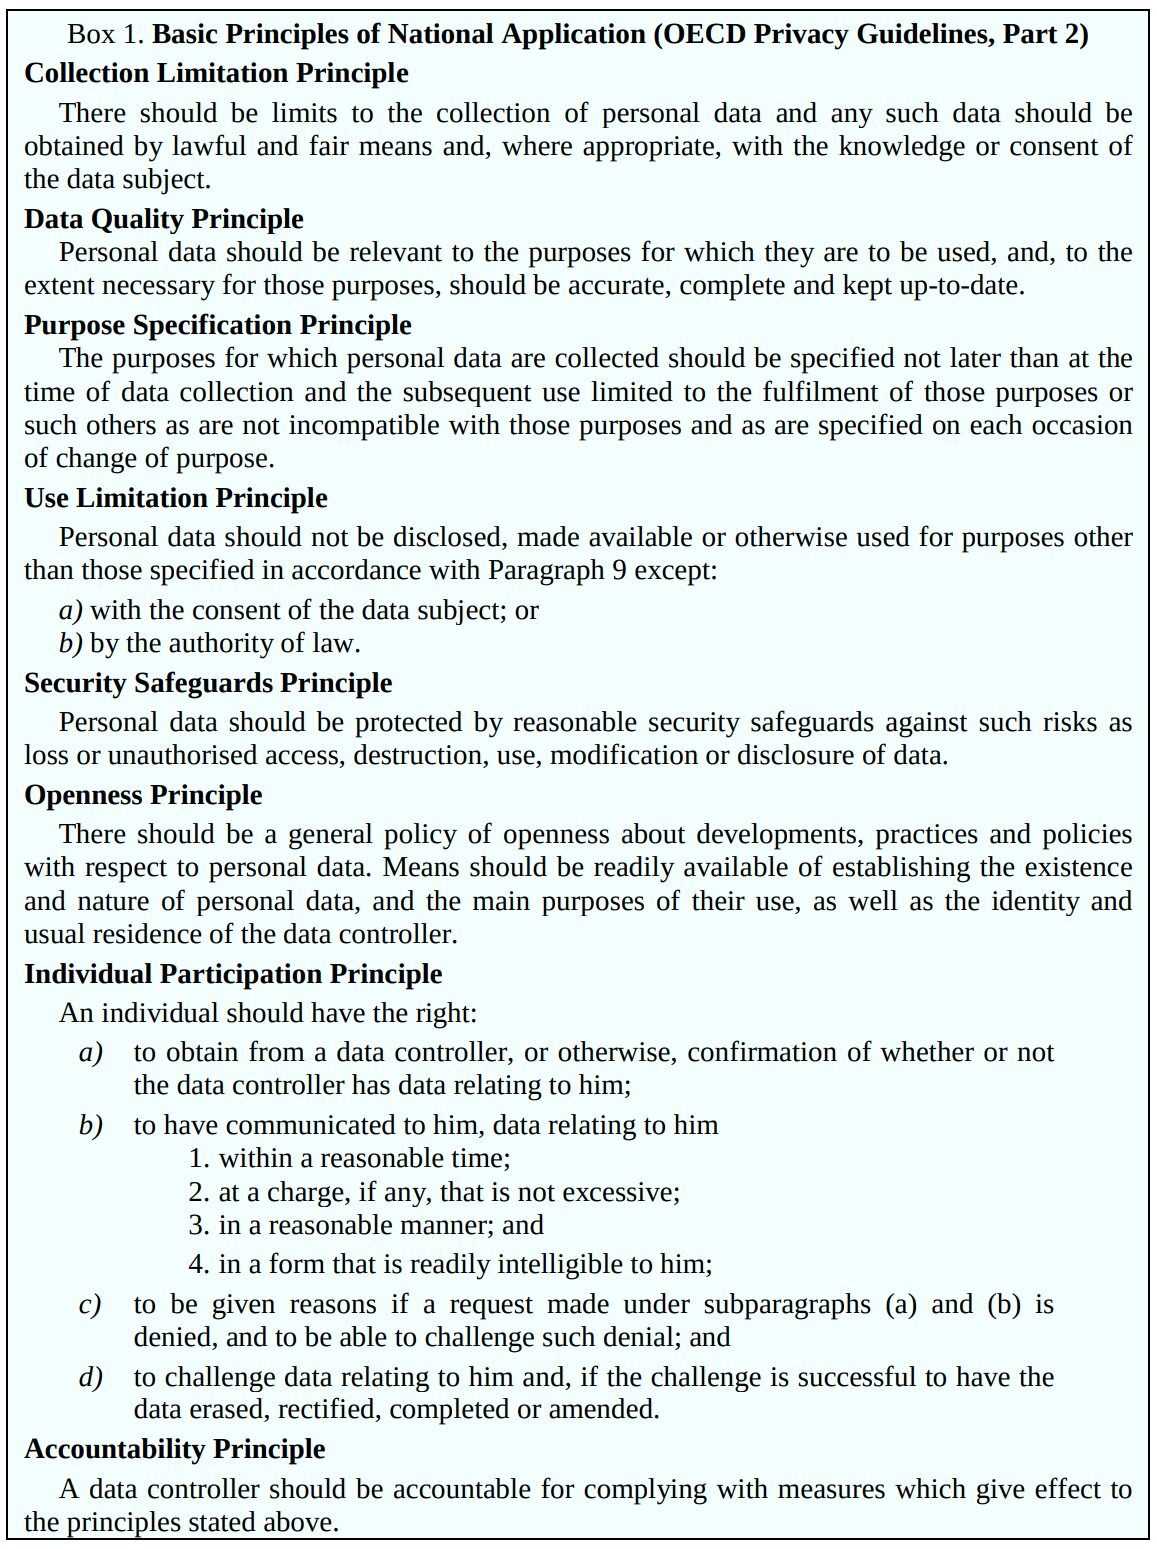
\includegraphics[width=\textwidth]{latex/figures/oecd_guidelines.jpg}
            \caption[OECD guideline]{OECD guideline \cite{oecd_oecd_2013}}
            \label{fig:oecd_guide}
        \end{figure}
        The first principle is the Collection Limitation Principle. It states that "There should be limits to the collection of personal data [..]" \cite{oecd_oecd_2013}. This principle is reflected in NIST's \textit{Guide to protecting the confidentiality of Personally identifiable information} \cite{mccallister_guide_2010}. In there, it is recommended to minimize the use, collection, and storage of personal data to the minimum necessary to serve its purpose.
        That way, the damage done on a possible data breach is minimized. It is also recommended to review the previously collected PII. If it is no longer relevant, it should be removed \cite{mccallister_guide_2010}.\\
        To protect data sets, the NIST guide also recommends the de-identification of information. Data with enough PII removed or obscured is treated as de-identified. One-way cryptographic functions (hash functions) may be used for this purpose \cite{mccallister_guide_2010}.\\
        Suppose there is no code or other association to re-identify the information is defined as anonymized \cite{mccallister_guide_2010}. This matches with the definition of anonymity and anonymization.


    \newpage
    %
    %%%%%%%%%%%%%%%%%%%%%%%%%%%%%%%%%%%%%
    %%%%%%%%%%%% Subsection %%%%%%%%%%%%%
    %%%%%%%%%%%%%%%%%%%%%%%%%%%%%%%%%%%%%
    %
    \subsection{Regulations}
        \label{subsec:related:law}
        Anonymity is defined by DIN EN ISO/IEC 29100 as an information characteristic that does not allow the identification of a person directly or indirectly \cite{german_institute_for_standardization_din_2020}. It furthermore declares anonymization as a process in which personally identifiable information is irrevocably transformed. This transformation denies the ability of an entity to identify a person indirectly or directly by itself or in cooperation with another entity \cite{german_institute_for_standardization_din_2020}.\\
        
        A major advantage of anonymized data is the exclusion of the GDPR legislation. Recital 26 of the regulation excludes anonymized data explicitly.\\ 
        "The principles of data protection should therefore not apply to anonymous information, namely information which does not relate to an identified or identifiable natural person or to personal data rendered anonymous in such a manner that the data subject is not or no longer identifiable. This Regulation does not therefore concern the processing of such anonymous information, including for statistical or research purposes." \cite{european_union_regulation_2016}\\
        Compared to the EU, the US have a wide range of privacy state laws. While the EU aims to provide one general regulation, the US privacy laws are split over four major regulations.
        These four are the \textit{Health Insurance Portability and Accountability Act} (HIPAA), \cite{rights_ocr_summary_2009}, which regulates healthcare provider, \textit{NIST 800-171} \cite{ross_protecting_2015}, which defines how to handle controlled unclassified information in non-federal information systems, the \textit{Gramm-Leach-Bliley Act (GLBA)} \cite{noauthor_gramm-leach-bliley_2013}, protecting personal information stored by financial institutes and the \textit{Federal Information Security Management Act (FISMA)} \cite{carper_s2521_2014} in which the requirements are stated for federal agencies information security programs. On top of these, states have additional privacy laws, which may be up to the GDPRs protection, depending on the state \cite{andrada_coos_eu_nodate}.\\
        The European data protection regulation provides a strong set of rules. These may be aggravated by member state laws but not weakened. This allows for even stronger data protections in some European countries.
        
    %
    %%%%%%%%%%%%%%%%%%%%%%%%%%%%%%%%%%%%%
    %%%%%%%%%%%% Subsection %%%%%%%%%%%%%
    %%%%%%%%%%%%%%%%%%%%%%%%%%%%%%%%%%%%%
    %
    \subsection{Private Data Publication}
        \label{subsec:related:private_data_analysis}
    
        \subsubsection{\textit{k}-anonymity}
            \label{subsec:related:kanon}
            To avoid the identification of a user, based on the published data and its attributes, record linkage should not be possible. Therefore a system design should consider the so-called quasi identifier (QI). These quasi identifiers may allow to draw a connection between the data set and an external source \cite{sweeney_k-anonymity_2002}.
            If a set of attributes is contained in an external release that might contain PII and contained in a released data set, these sets of attributes are called quasi identifiers, as it allows the linkage between these two data sets.
            If a data set S has $QI_S$ associated with it, S satisfies \textit{k}-anonymity if each sequence of values S[$QI_S$] appears at least \textit{k} times. 
        	In addition, each sequence S[$QI_S$] needs to belong to a different user.
        	This does protect the data set against linking by using direct matching, as Sweeny proposes in  \cite{sweeney_k-anonymity_2002}.\\
            One of the shortcomings of \textit{k}-anonymity is that each tuple of attributes needs to belong to a different user, as Fung demonstrates in  \cite{fung_introduction_2011}, as they are possibly expose sensitive data otherwise.

        \subsubsection{\textit{l}-diversity}
            \label{subsec:related:l-div}
            In  \cite{machanavajjhala_l-diversity_2007} Machanavajjhala et al. shows that k-anonymity is susceptible to the two attack vectors: homogeneity and background knowledge.
            The homogeneity attack works on datasets with groups that lack diversity in sensitive attributes. The background knowledge attack on the other hand uses available knowledge in addition to the provided dataset that is not directly matched to attributes.\\
            Machanavajjhala et al. introduce the \textit{l-}diversity framework to counter these weaknesses by requiring that the values of a sensitive attributes are well represented in each group. \textit{l}-diversity is not intended to replace \textit{k}-anonymity, but to extend it and improve privacy that way  \cite{machanavajjhala_l-diversity_2007}.
            

        % differential privacy
        \subsubsection{Differential Privacy}
            \label{subsec:related:dif_privacy}
            Differential privacy (DP) is a property of the data access mechanism and unrelated to auxiliary information available \cite{dwork_algorithmic_2013}. 
            It promises that the addition or removal of a single dataset to an existing database does not affect the outcome of an analysis with a strong mathematical definition of privacy. A protection against privacy attacks like re-identification, record linkage, and differencing is mathematically provable provided  \cite{agrawal_differential_2008},  \cite{wood_differential_2018}. \\
            This guarantees that anyone will make the same inference about an individual's PII or private information whether the individual's dataset was included in the analysis or not \cite{wood_differential_2018}. Therefore making post-processing impossible as an analyst can not make the output less differential private without additional knowledge of the private database \cite{nguyen_understanding_2019}.
            
%%%%%%%%%%%%%%%%%%%%%%%%%%%%%%%%%%%%%
%%%%%%%%%%%%%%%%%%%%%%%%%%%%%%%%%%%%%
%%%%%%%%%%%%   SECTION   %%%%%%%%%%%%
%%%%%%%%%%%%%%%%%%%%%%%%%%%%%%%%%%%%%
%%%%%%%%%%%%%%%%%%%%%%%%%%%%%%%%%%%%%
\section{Data Transmission}
    \label{sec:related:data_transmission}
    %
    The Tor Project is probably the most known approach for anonymized data transmission over the Internet. Besides Tor, we will discuss different approaches to transmit data over a network. In \ref{subsec:related:overlay} the Tor and I2P overlay network are going to be discussed, followed by the domain name system in section \ref{subsec:related:dns}. 
        
        
    %
    %%%%%%%%%%%%%%%%%%%%%%%%%%%%%%%%%%%%%
    %%%%%%%%%%%% Subsection %%%%%%%%%%%%%
    %%%%%%%%%%%%%%%%%%%%%%%%%%%%%%%%%%%%%
    %
    %%%% Overlay Networks
    %
    \subsection{Overlay Networks}
        \label{subsec:related:overlay}
        %
        Several overlay networks provide different functionalities. Caching overlays enhance the serving of static content. Routing overlays provide different features for dynamic content than the underlying networks and security overlays, that improve the security of networks and can help mitigating distributed denial of service (DDoS) attacks \cite{pathan_overlay_2014}.\\
        Two overlay networks will be discussed. On the one hand, there is Tor \cite{dingledine_tor_2004}, on the other, I2P \cite{zantout_i2p_2011}. Both systems aim to enhance the anonymity of the internet by adding additional layers.\\
        Furthermore, additional protocols like P5 \cite{sherwood_p_2005} and Herbivore \cite{goel_herbivore_2003} have been reviewed. As they are similar to the presented solutions, but are less known or require additional implementation steps or infrastructure, they are not described in this section.
     
     
    %%% Tor %%%
    \subsubsection{Tor}
        The so-called Onion Routing used  by Tor is a distributed overlay network to anonymize TCP-based applications. On its path from sender to receiver, each step in the network only knows its predecessor and successor. Therefore information is layered and secured with symmetric keys, which are unwrapped at each step, like the layers of an onion.
        Tor provides perfect forward secrecy by negotiating session keys with each successive hop. If one hop gets compromised, after the keys are deleted, old traffic can't be decrypted \cite{dingledine_tor_2004}, \cite{borisov_shining_2008}.\\
        Tor requires additional work on the client site to configure and set up. 
        The network is operated by a wide variety of people and organizations.
        Thousands of relay nodes are used to route traffic from the origin to the receiver. It was in 2009 and is of today the biggest network designed for anonymity in operation \cite{edman_anonymity_2009}.
        Therefore it is independent of the collecting entity. Tors systems provide anonymity for the sender against the server and an attacker in most cases \cite{arma_one_2009},  \cite{poulsen_feds_2013}, \cite{samson_tor_2013}, \cite{herrmann_website_2009}.\\
        The use of the Tor network is free of charge. It is open source software, but connecting to it requires additional setup steps from the user. To route only traffic of one application through the Tor network, configuration files need to be adjusted and additional software installed. As the Tor network is spread around the globe and no path can, or should, be provided, delay and latency increase, if the tor network is used for all applications on the device. Also the available resources would be reduced for tasks that are not required to have an extended privacy protection.\\
    
    
    
    %%% I2P %%%
    \subsubsection{The Invisible Internet Project - I2P}
        I2P is an overlay network with privacy-by-design in mind intended to connect services within a closed network.
        Exit proxy servers are available but not recommended by the developer. Within the network, nodes can communicate in any way they want. I2P is free open source software and can be added to a regular web service to make it available on the closed network. Each network node has unidirectional inbound and outbound tunnels, and every node is visible on the network. However, the traffic of a node can not be seen by other network participants. The network is decentralized and uses distributed hash tables for a network database and contact information security \cite{i2p_intro_2014}.\\
        To contact another client, a message is sent out through its own outbound tunnel, trying to reach the other client's inbound tunnel. Each client can choose the tunnels' length to find a trade-off between latency and anonymity \cite{anoncoin_i2p_2018}.\\
        I2P requires additional software or setup steps on the client and server-side to access the network.\\
        
        
        
    
    %%% VPN %%%
    \subsubsection{Virtual Private Network - VPN}
        A VPN provides an encrypted connection from the user's system to an exit point, the VPN server. For further communication, the IP address of the VPN server is used. This may change the country of origin and prevent things like geoblocking or other restrictions imposed by the internet service provider \cite{microsoft_virtual_2009}.\\
        A VPN provides privacy against prying eyes in the path from the client to the VPN server. It also provides anonymity to the web service requested. Virtual private networks can be self-hosted, hosted by a for-free or paid provider. Additional steps, like configuration, are required on the user's end to use it.\\

    
    %%%%%%%%%%%%%%%%%%%%%%%%%%%%%%%%%%%%%
    %%%%%%%%%%%% Subsection %%%%%%%%%%%%%
    %%%%%%%%%%%%%%%%%%%%%%%%%%%%%%%%%%%%%
    %
    %%%% Special systems
    %
    \subsection{Special Systems}
        \label{subsec:related:special}
        There are already systems available that have been designed for anonymized data collection and transmission. 
        Two such systems currently in use by major open source web browsers are dissected below. In \ref{subsec:related:dns} the domain name system is discussed. It is usually not connected to anonymous data transmission but provides a reliable way to disconnect the sender's IP address from the DNS query.
        %
        
    %%% Prochlo %%%
    \subsubsection{Prochlo}
        Prochlo describes a system architecture for large-scale monitoring of software usage activities. The system uses an "Encode, Shuffle, Analyze" approach. Thereby data is encoded and encrypted on one side. It's also the encoder's objective to add noise and take care of the randomness of the collected data \cite{bittau_prochlo_2017}.\\
        Afterwards, the data is transmitted to a centralized shuffler. They are responsible for the masking of the data origin by removing metadata (IP address, order, and time of arrival).
        The data is held for a prolonged time and transmitted only when a single data item is hidden in a crowd of similar data items. Therefore shufflers need to be trusted entities and separated from the analyzer \cite{bittau_prochlo_2017}. To add further trustworthiness, they should be run by a third party. The aggregated and reordered data is sent out at random intervals to further increase the decoupling of the time of arrival and enhance the privacy of clients.\\
        After transmission, the data is decrypted, stored, and aggregated by the analyzer. 
        Added noise and fragmentation on the encoder side, as well as shuffling, may be sufficient to provide differential anonymity in this system.
        
        Prochlo is developed by Google and used by Chromium and, in modified form, by Brave.
        \begin{figure}[hb]
            \centering
            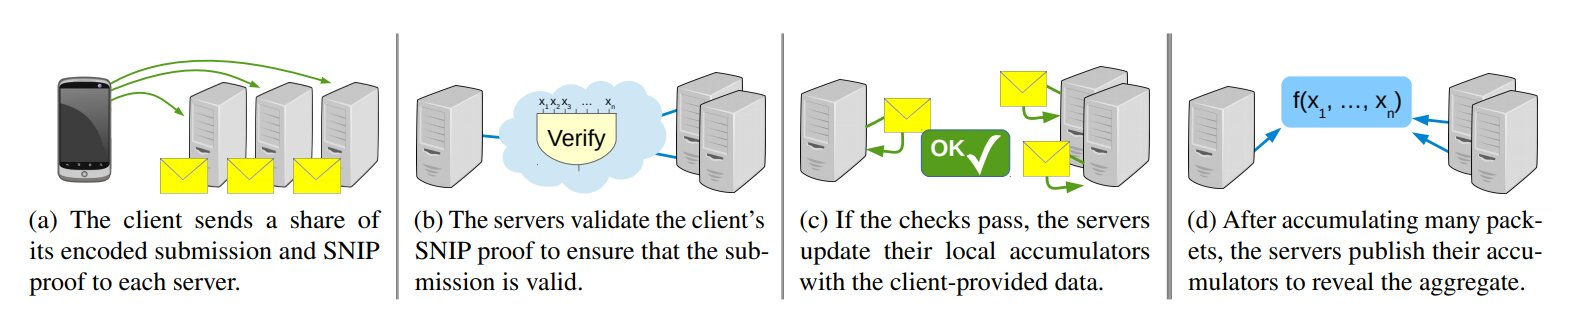
\includegraphics[width=\textwidth]{latex/figures/prio_overview.jpg}
            \caption[Overview of Prios processing pipeline]{Overview of Prios processing pipeline \cite{corrigan-gibbs_prio_2017}}
            \label{fig:prio_overview}
        \end{figure}
    
    %%% Prio
    \subsubsection{Prio}

        Prio was developed by Corrigan-Gibbs et al. \cite{corrigan-gibbs_prio_2017} in 2017 as a privacy-preserving system for collecting aggregated statistics.
        It was developed at Stanford University's Computer Science department for nonsensitive data already covered by their Telemetry tool. 
        Prio splits the collected client data into shares. 
        The parts are sent to different servers and aggregated with shares of other users before being published (see figure \ref{fig:prio_overview}) \cite{corrigan-gibbs_prio_2017}.\\
        The system promises privacy as long as one of the servers is honest, therefore providing strong cryptographic privacy. A limited form of robustness is provided as long as all servers are honest. It can detect and discard syntactically incorrect client data while preserving the privacy of the data. However, Prio can not prevent a client from sending in-range data, that is untrue \cite{corrigan-gibbs_prio_2017}.\\
        It is in experimental use by Firefox Origin Telemetry \cite{englehardt_next_2019}.
        
        
    %%% DNS 
    \subsection{Domain Name System - DNS}
        \label{subsec:related:dns}
        The Domain Name System is hierarchically and decentralized designed to allow systems connected to a network to translate memorable domain names into IP addresses \cite{stevens_tcpip_1993}.\\

        This translation is needed before an application can request a TCP connection or send UDP datagrams. A domain name is a list of labels separated by dots. 
        Each label can have a length of up to 63 bytes, with a maximum length of the requested domain of 255 bytes \cite{stevens_tcpip_1993}.\\
        The dot is used to separate each layer in a domain but is also the internet root, which terminates all Fully Qualified Domain Names (FQDN), but is often omitted \cite{jeftovic_managing_2018}.
        In figure \ref{fig:dns_tree} it is shown how a hostname can be separated and traversed.
        The first field, following the, here omitted, root entry is the so-called Top-Level Domain (TLD). In figure \ref{fig:dns_tree} this would be "com". The root and top-level domain are required to find the responsible authoritative nameserver for any related query \cite{jeftovic_managing_2018}.

    	\begin{figure}[h!]
    	    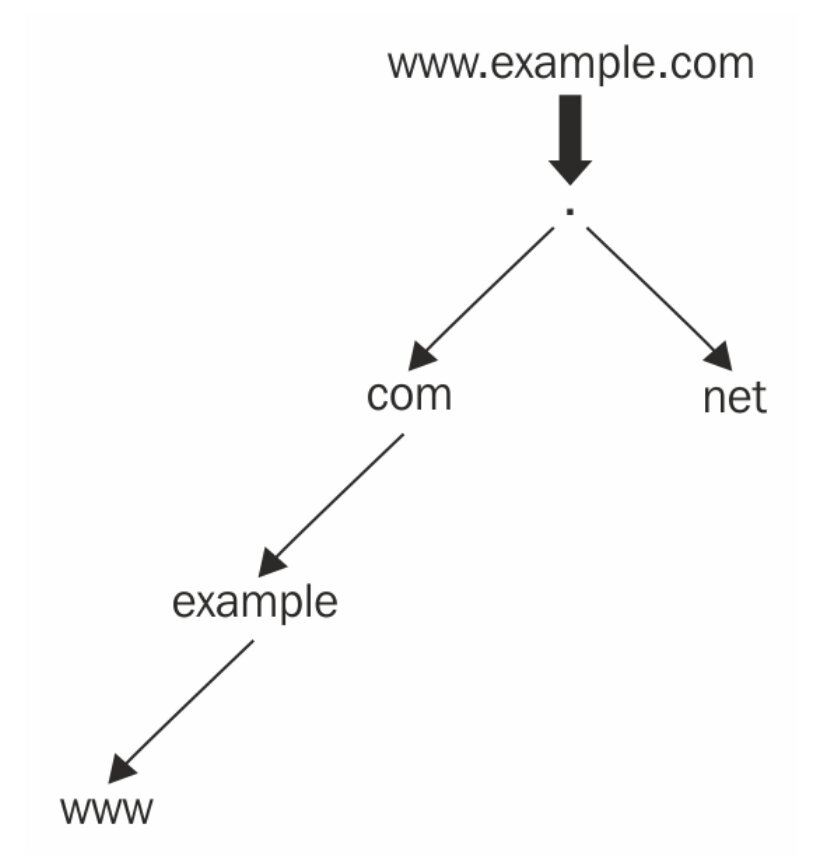
\includegraphics[width=\textwidth]{latex/figures/domain_name_tree.jpg}
    	    \caption[Domain Name Tree for www.example.com.]{Domain Name Tree for www.example.com. \cite{jeftovic_managing_2018}}
    	    \label{fig:dns_tree}
        \end{figure}

        The name system is structured in non-overlapping zones, as shown in the right segment in figure \ref{fig:dns_query} with the root domain on top \cite{herrmann_beobachtungsmoglichkeiten_2016}.
        A server containing all information about a subset of the namespace is called an authoritative server. To extract the information from the authoritative server, a so-called resolver is used \cite{friedewald_privacy_2018}.
        As the hierarchical structure of the domain name system provides sender anonymity, meaning the receiver does not know the source of the message, the system can be used to transmit data anonymously to a collecting server. This can be achieved without any further additions to the protocol or configuration on the client-side.
        Advanced techniques like DNS over HTTPS (DoH) \cite{ermert_cloudflare_2020} \cite{mcmanus_dns_2018} or DNS Security Extensions (DNSSEC) \cite{larson_dns_2005} can be used.\\
        DoH uses transport layer security (TLS) to encrypt a connection to a proxy server, which then transmits the DNS request. That way, the proxy server is the only participant who knows the sender's IP address. DNSSEC can add another layer of security in protecting against attacks like DNS cache poisoning by adding new components to the DNS system that check the integrity and authentication of DNS data.\\
        The newly presented Oblivious DNS over HTTPS (ODoH) developed by Apple, Fastly, and Cloudflare may add additional privacy to every DNS query and removes one weakness from DoH \cite{verma_improving_2020}.\\
        In ODoH, the client encrypts its DNS request for a target server and sends this encrypted message to the proxy server, which then relays the message to the target server. This procedure removes the original request from the client's IP, making the proxy unaware of it.
        At the same time, the target server only knows the IP of the proxy as the source. The response is then encrypted for the client and relayed back through the proxy \cite{verma_improving_2020}.
        
        
        
        %%% TODO: citation for DOH and DNSSec
        
        \begin{figure}
            \centering
            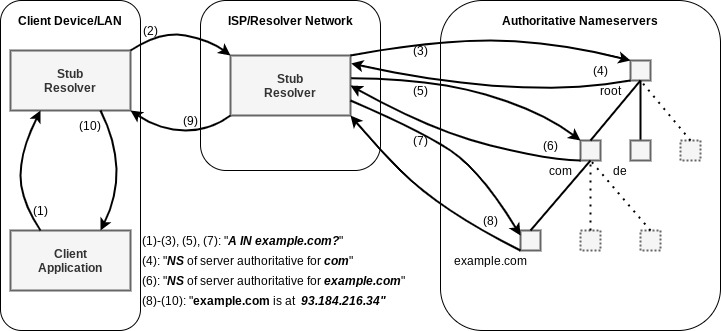
\includegraphics[width=\textwidth]{latex/figures/dns_resolve.jpg}
            \caption[DNS Query with resolver for example.com]{DNS Query with resolver for example.com, based on \cite{friedewald_privacy_2018}}
            \label{fig:dns_query}
        \end{figure}
        
        
        The DNS is also used in malware for DNS tunneling or data exfiltration.
        In DNS tunneling domain TXT records are used to initiate a session with a command and control server. The TXT field can also contain instructions for the malware \cite{das_detection_2017}.\\
        To exfiltrate data in a DNS request, the information in question is Base32 encoded and split into 63 byte sized chunks. Afterwards, requests are started to a monitored or controlled domain with the encoded data as fields \cite{mertens_infosec_2017}.\\
        
\newpage
%%%%%%%%%%%%%%%%%%%%%%%%%%%%%%%%%%%%%
%%%%%%%%%%%%%%%%%%%%%%%%%%%%%%%%%%%%%
%%%%%%%%%%%%   SECTION   %%%%%%%%%%%%
%%%%%%%%%%%%%%%%%%%%%%%%%%%%%%%%%%%%%
%%%%%%%%%%%%%%%%%%%%%%%%%%%%%%%%%%%%%
\section{Related Software}
    \label{sec:related:related_sw}
    %
    This section introduces some open source projects that allow data collection or actively collect user-system information. 
    
    %%% Ubuntu %%%
    \subsection{Ubuntu}
        Ubuntu is one of the best-known distributions of the GNU/Linux Operating system. It provides several packages for server, desktop, or embedded usage. It is used by many major companies on their server \cite{canonical_enterprise_nodate}\\
        Ubuntu collects data with its "ubuntu-report" tool. By default, a system reports its data only once per distribution version. The tools provide a graphical user interface and command-line version and prompt the user's information before sending \cite{roche_ubuntuubuntu-report_2020}.\\
        A JSON report, as shown in listing \ref{lst:ubuntu-report} in the Appendix, is sent to the Ubuntu server if the user opts in. If the user opts out, a report is created as in listing \ref{lst:opt-out} and sent to the Ubuntu server \cite{roche_ubuntuubuntu-report_2020}.\\ 
        \begin{lstlisting}[language=json, caption=JSON report on opt out, label=lst:opt-out]
            {
                "OptOut": true
            }
        \end{lstlisting}
        This allows Canonical to get a relatively precise number of internet-connected devices that run Ubuntu.\\
        There is no PII collected. Only data like system architecture, RAM, disk space, monitor count, and resolution are reported.\\
        An HTTP POST is sent over TLS to the Ubuntu server to transmit the data.\\
        
        In an HTTP POST, the body of the message contains the payload, compared to a GET, where the payload is appended to the URL.
        It is not encrypted or encoded by default but can be upfront to protect the body's data from inspection. Protocols like TLS can be used to encrypt the transport. But if an attacker knows the session key, all ongoing communication can be read. Prior communication is secured as TLS provides forward secrecy.\\
        
        As this is a TCP direct connection, the public IP address of the sending system can be connected to the collected data on the server-side.
        The user must trust the collecting services, that the information is not stored but discarded.\\
        
    %%% hw-probe %%%
    \subsection{Hardware Probe Tool - hw-probe}
        The Hardware Probe Tool is an open source tool to collect hardware, system, and log information on Linux and BSD-based systems. It is written in Perl, and collected data is available for everyone to see. 9780 unique systems reported their system information in 2019 \cite{ponomarenko_linux_nodate}.
        While serial numbers and MAC addresses are collected, they are salted and hashed with SHA512, and only 32 bytes are transmitted. With salting, additional (random) data is added to the original message to increase the effort for reidentification attacks.
        This should avoid the recreation of any personal identifiable information and uniquely identify a system against the database  \cite{project_linuxhwhw-probe_2020}.\\
        The collected data can be pretty extensive if a complete collection is enabled. It includes, among other things, installed drivers, connected PCI devices, system architecture, operating system, network interface type, and UUID \cite{project_linuxhwhw-probe_2020}.\\
        
        HTTP POST messages are sent to the collection server to transmit the collected data. The transmission uses TLS to secure the content of these messages \cite{project_linuxhwhw-probe_2020}.\\
        Again the IP of the system is connected to the data set transmitted, and the user has to rely and trust on the collecting entity to separate this two information from each other.\\
    


\newpage
    %%% Firefox %%%
    \subsection{Firefox}
        Firefox is a browser that promises speed and privacy. It provides advertisement and tracker blocking. Besides, it is available on all major platforms \cite{mozilla_corporation_download_nodate}.\\ 
        By default, Firefox collects a wide range of data. These data collections are called Pings. Each Ping contains a certain type of information. There are at least 27 different Ping types in use at the time of writing \cite{mozilla_telemetry_nodate}.
        
        \begin{wrapfigure}{R}{0.41\textwidth}
            \centering
            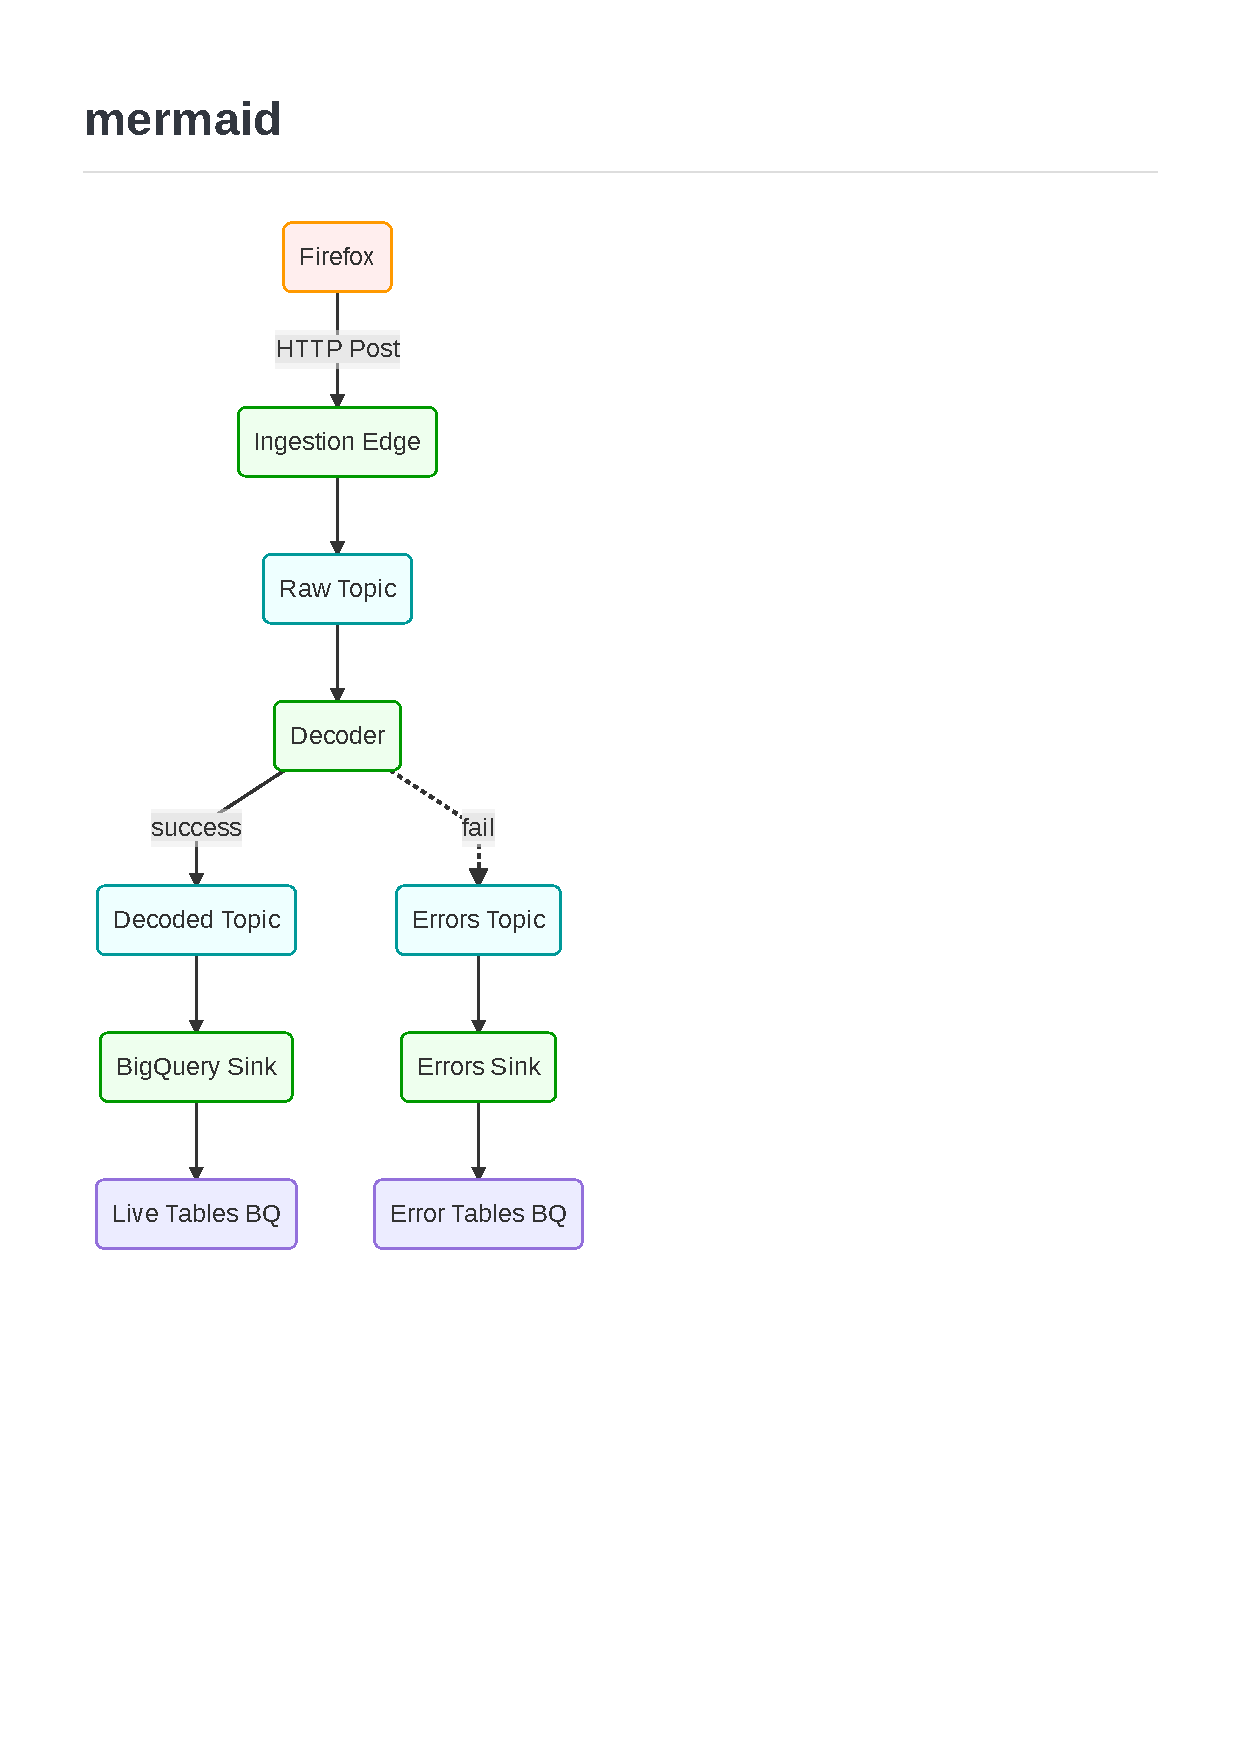
\includegraphics[clip, trim=0.5cm 8cm 8cm 3.5cm, width=0.4\textwidth]{latex/figures/firefox_telemetry_graph}
            \caption[Firefox data flow]{Firefox data flow based on  \cite{mozilla_overview_2020}}
            \label{fig:moz_data_flow}
        \end{wrapfigure}
        
        The "main" Ping is used for most telemetric data. It contains extensive health and performance information on Firefox, but also most system information. The JSON structure of a "main" Ping can be seen in Mozillas pipeline schema GitHub repository \cite{mozilla_mozilla-servicesmozilla-pipeline-schemas_2020}. 
        Besides information on CPU, GPU, and operating system, it contains information on installed add-ons and the reason for sending the Ping.
        It is sent at least every 24 hours, but also on startup and other occasions. While basic telemetry, like the main ping, can be disabled on the settings page, Firefox will still send selected Pings to its server unless disabled in \textit{about:config}.
        %TODO: verify with wireshark - firefox sends stupid amount of data
        To send the collected Telemetry, Firefox uses a program called Ping Sender.
        This will send an HTTP POST to the Edge Server, where it is forwarded to the data pipeline, if formatted correctly.
        If a client IP address is available at the decoder, the geolocation will be determined and saved.
        The IP address gets discarded from the data set in the process \cite{mozilla_overview_2020}, \cite{mozilla_http_2020}, \cite{firefox_ping_nodate}.\\
        A reduced data pipeline can be seen in figure \ref{fig:moz_data_flow}.
        
        
        
    
        Mozilla was experimenting with Prio in 2018, \cite{helmer_testing_2018}, and based on the experiment they developed Firefox Origin Telemetry  \cite{englehardt_next_2019} which is, at the time of writing, in use only for content blocking and still experimental \cite{noauthor_origin_nodate}.\\
    
    
    %%% Brave %%%
    \subsection{Brave}
        Brave is a free open source browser with a focus on privacy. It provides advertisement and tracker blocking, as well as a Tor integration. It is based on Chromium and promises to be faster. It also claims to have better default privacy than Firefox. It is a relatively new Browser but already supports all major platforms \cite{brave_secure_nodate}.\\
        Brave uses a technique called Privacy Preserving Product Analytics (P3A) for telemetry data, which can be turned off at any time.
        They claim that their P3A does cover way more than expected by GDPR. No personally identifiable data (PII) is collected or transmitted \cite{brave_privacy-preserving_2019}.\\
        Therefore Braves telemetry process is split into two phases. The first phase consists of several multiple-choice questions, for which the answer is sent individually.
        Each question poses a number of answers. Quantifiable questions, like the number of open tabs, provide ranges for each answer for enhanced privacy \cite{brave_privacy-preserving_2019}. These Questions and possible answers can be reviewed in Braves GitHub repository \cite{brave_software_inc_brave-browser_2019}.
        The questions of phase one can be seen in listing \ref{lst:brave-report} in the appendix.\\
        At a randomized time after opening the browser, the number of open tabs is counted and send out once an hour with further information \cite{brave_privacy-preserving_2019}.
        An answer contains:
        \begin{itemize}
            \item Question number, Answer number
            \item OS/Platform
            \item Release information (nightly/dev/bet/release)
            \item Week of installation (if the installation was within 90 days)
            \item Country (if fewer than 6000 installs per week, this is removed)
            \item Referral code (only if within 90 days of install and referrer is big enough)
        \end{itemize}
        Every answer is sent to Braves content delivery network (CDN) and stripped of the IP address of the client at the edge of the CDN \cite{brave_privacy-preserving_2019}.
        . 
        The Second Phase uses a protocol based on Prochlo (see \ref{sec:related:data_transmission}). 
        
        The study Leith conducted in February 2020  \cite{leith_web_2020} supports the claims made by Brave for a privacy caring browser.\\
        In his survey, Leith evaluated the privacy settings of six browsers (Brave, Chrome, Edge, Firefox, Safari, and Yandex). While Brave and Firefox (with changed defaults) were strongly focused on privacy, all Browsers did send their reports combined with the user's IP address \cite{leith_web_2020}.
        This is problematic, as an IP address can be used to pin down the user's geolocation \cite{koch_geolocation_2013}. Workplaces or homes can be derived based on the time people spend in places during the day or night. 
        While Brave Software Inc. claims that they remove the IP address at the edge of their CDN, the user has to trust the CDN operator to strip the send data of the address for phase one answers. In phase two, the user has to trust the shuffler to remove the metadata from the collected data. 
\newpage

%%%%%%%%%%%%%%%%%%%%%%%%%%%%%%%%%%%%%
%%%%%%%%%%%%%%%%%%%%%%%%%%%%%%%%%%%%%
%%%%%%%%%%%%   SECTION   %%%%%%%%%%%%
%%%%%%%%%%%%%%%%%%%%%%%%%%%%%%%%%%%%%
%%%%%%%%%%%%%%%%%%%%%%%%%%%%%%%%%%%%%
\section{Summary}
    In this chapter, we discussed what personal information is and how it should be handled.
    In addition, we summarized previous work on related topics. This allows us to narrow our research.
    Prio and Prochlo require additional infrastructure. As open source organizations are usually underfunded, every additional server leaves a dent in the budget. Therefore these systems may be
    useful for organizations with sufficient funding, but not for small projects. Some of the mentioned systems in this chapter depend on the user's trust that their transmission information is stripped from the data.\\
    
    On the other hand, client-side enabled anonymization, like using the tor network or VPNs, may require additional maintenance or knowledge from the user. This could reduce the amount of participating users significantly.\\
    
    The Domain Name System provides a hierarchical structure that strips the sender's information from the transmitted data in a reliable way. A user can trust the DNS to remove its IP and does not depend on an organization to handle that properly. Furthermore the anonymization process does not require any additional knowledge.\\
    Utilizing DNS for data transmission opens up a range of new issues, like plain text data transmissions. These issues need to be handled and will be discussed in the next chapter.\\ 

%


  